\section{PETSc Finite-Element Implementation}

Formulating the weak form of the governing equation in terms of
point-wise functions allows the PyLith implementation of the equations
to be done at a rather high level. Most of the finite-element details
are encapsulated in PETSc routines that compute the integrals and
solve the system of equations. In fact, adding materials and boundary
conditions requires calling only a few PETSc finite-element functions
to register the point-wise functions. A new material may need to add
to the library of solution subfields and auxiliary subfields, but
adding these fields is also done at a high-level.

The remainder of this section discusses three aspects of the
finite-element implementation handled by PyLith to give you a peek of
what is doing on under the hood.

%\subsection{Meshing}

%We employ the \textit{cohesive element} formulation for faults in
%order to apply separate constitutive relations to the fault
%surface. We want the two sides of the faults to operate independently
%in some sense, but maintain a coupling (prescribed slip or spontaneous
%rupture). In other words, we would like the displacement of the two
%sides to be independent variables, constrained by the coupling
%equation. Alternatively, we could have maintained the same mesh
%topology, but added extra variables on the vertices, edges, and faces
%on the fault surface. However, this would change assembly on all cells
%along the fault, and greatly complicate optimization and maintenance
%of the assembly code. Instead, we pushed the complication of the fault
%interface to the mesh topology.

\subsection{\object{DMPlex}}

The finite-element mesh is stored as a \object{DMPlex} object. This is
a particular implementation of the PETSc Data Management (\object{DM},
renamed \object{PetscDM} within PyLith) object. Within a
\object{DMPlex} object vertices, edges, faces, and cells are all
called points. The points are numbered sequentially, beginning with
cells, followed by vertices, edges, and then faces. Treating all
topological pieces of the mesh the same way, as points in an abstract
graph, allows us to write algorithms which apply to very different
meshes without change. For example, we can write a fintie element
assembly loop that applies to meshes of any dimension, with any cell
shape, with (almost) any finite element.

\subsubsection{Point Depth and Height}

In general, vertices are at a \textit{depth} of 0 and cells are at the
maximum depth. Similarly, cells are at a \textit{height} of 0 and
vertices are at the maximum height. Notice that depth and height
correspond to the usual dimension and
codimension. Table~\vref{tab:dmplex:height:depth} shows the heights
and depths of the vertices edges, faces, and cells in a 3-D mesh.

\begin{table}[htbp]
  \caption{Depth and height of various topological pieces.}
  \label{tab:dmplex:height:depth}
  \begin{center}
    \begin{tabular}{lcc}
      \hline
      Point type & Depth & Height \\
      \hline
      Vertices  &  0  &  3 \\
      Edges  &  1  &  2 \\
      Faces  &  2  &  1 \\
      Cells  &  3  &  0 \\
      \hline
    \end{tabular}
  \end{center}
\end{table}

For a boundary mesh, we currently store the full set (vertices, edges,
faces, and cells). Obviously for 2-D meshes, the boundary mesh doesn't
contain "volume" cells, but just vertices, edges, and faces. This
means the "boundary" cells are at a height of 1 and a depth equal to
the maximum depth $-$ 1 .

\begin{figure}
  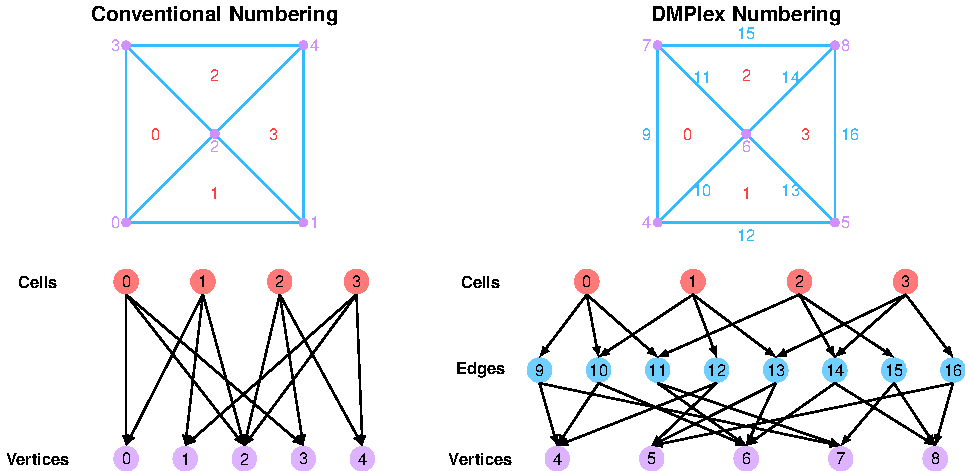
\includegraphics{developer/figs/meshtopology}
  \caption{Conventional numbering (left) with vertices and cells numbered independently and \object{DMPlex} numbering (right)
  with cells, vertices, edges, (and faces), numbered sequentially.}
  \label{fig:developer:mesh:topology}
\end{figure}

\subsection{\object{PetscSection} and \object{PetscVec}}
\label{sec:developer:petsc:section}

We store a field over the mesh in a vector (PETSc \object{Vec} object,
renamed \object{PetscVec} in PyLith). The \object{PetscSection} object
describes the layout of the vector over the DMPlex object. The vector
may hold multiple subfields, each with its own discretization. The
chart of the \object{PetscSection} defines the range of points
(minimum and maximum) over which the section is defined. For each
point in the chart, the section holds the number of degrees of freedom
a point has and the offset in the \object{PetscVec} for its first
degree of freedom. The section also holds the number of
degrees of freedom and offset for each individual subfield within the
section for each point in the chart.

Because the \object{PetscSection} knows only about points, and not
about topolgoy or geometry, it allows us to express the mathematical
concepts without getting lost in the details. For example, a $P_1$ 3D
vector field assigns 3 dofs to each vertex. This same section could be
used to layout a field over a circle, surface of a cylinder, M\"obius
strip, sphere, cube, ball, or Pylith mesh. It separates the layout of
data over a mesh from the actual storage of values, which is done by
the \object{PetscVec}. The section tells you how to look up the
values, which are associated with a piece of the mesh, inside the
vector. For example, you can ask for the offset into the vector for
the values associated with an edge in the mesh, and how many dofs
there are on the edge.

The \object{PetscSection} also includes the information about the
constrained degrees of freedom. We refer to a \object{PetscVec} that
includes the values for the constrained degrees of freedom as a {\em
  local} vector and a \object{PetscVec} with the values for the
constrained degrees of freedom removed as a {\em global}
vector. Constraints often arise from Dirichlet boundary conditions,
which change the basis functions of the approximating space, but can
also arise from algebraic relations between unknowns. A local vector
is used for assembly of the residual vector and Jacobian matrix,
because we need the boundary values in order to compute those
integrals. Global vectors are used for the algebraic solver because we
do not want solution values fixed by constraints to participate in the
solve.

\begin{shell}[\object{PetscSection} information for a solution field with three subfields]
# This example solution field has three subfields:
#   * displacement (vector field, 2 components, basis order 1)
#   * velocity (vector field, 2 components, basis order 1)
#   * pressure (scalar field, 1 component, basis order 0)
#
# The displacement and velocity subfields have degrees of freedom on the vertices.
# The pressure subfield has degrees of freedom on the cells.
#
# The order of the values (offsets in the PetscVec) follows the
# ordering of the points (cells, vertices, edges, and faces).
# In this example, the pressure subfield appears first (offsets 0-3),
# followed by the two components of the displacement subfield and
# velocity subfield for each point.
PetscSection Object: 1 MPI processes
  type not yet set
3 fields
  field 0 with 2 components # displacement field
Process 0:
# (POINT) dim SUBFIELD_NUM_COMPONENTS offset OFFSET
(   0) dim  0 offset   0 # Cells
(   1) dim  0 offset   0
(   2) dim  0 offset   0
(   3) dim  0 offset   0
(   4) dim  2 offset   4 # Vertices
(   5) dim  2 offset   8
(   6) dim  2 offset  12
(   7) dim  2 offset  16
(   8) dim  2 offset  20
(   9) dim  0 offset  24 # Edges
(  10) dim  0 offset  24
(  11) dim  0 offset  24
(  12) dim  0 offset  24
(  13) dim  0 offset  24
(  14) dim  0 offset  24
(  15) dim  0 offset  24
(  16) dim  0 offset  24
field 1 with 2 components # velocity field
Process 0:
(   0) dim  0 offset   0 # Cells
(   1) dim  0 offset   0
(   2) dim  0 offset   0
(   3) dim  0 offset   0
(   4) dim  2 offset   6 # Vertices
(   5) dim  2 offset  10
(   6) dim  2 offset  14
(   7) dim  2 offset  18
(   8) dim  2 offset  22
(   9) dim  0 offset  24 # Edges
(  10) dim  0 offset  24
(  11) dim  0 offset  24
(  12) dim  0 offset  24
(  13) dim  0 offset  24
(  14) dim  0 offset  24
(  15) dim  0 offset  24
(  16) dim  0 offset  24
field 2 with 1 components # pressure field
Process 0:
(   0) dim  1 offset   0 # Cells
(   1) dim  1 offset   1
(   2) dim  1 offset   2
(   3) dim  1 offset   3
(   4) dim  0 offset   4 # Vertices
(   5) dim  0 offset   4
(   6) dim  0 offset   4
(   7) dim  0 offset   4
(   8) dim  0 offset   4
(   9) dim  0 offset   4 # Edges
(  10) dim  0 offset   4
(  11) dim  0 offset   4
(  12) dim  0 offset   4
(  13) dim  0 offset   4
(  14) dim  0 offset   4
(  15) dim  0 offset   4
(  16) dim  0 offset   4


\end{shell}

\subsection{Integration}

Integration involves integrals over the domain or the boundary of the
domain. These two operations are done by different PETSc functions.

\begin{description}
\item[\object{DMPlexComputeResidual\_Internal}] Compute the
  contribution to the LHS or RHS residual for a single material. This
  function and the functions it calls handle looping over the cells in
  the material, integrating the weak form for each of the fields, and
  adding them to the residual.

  A more appropriate name would be
  \object{DMPlexComputeResidualSingle} although that may change once
  we have a separate \object{PetscDM} for each material.
%
\item[\object{DMPlexComputeBdResidualSingle}] Compute the contribution
  to the LHS or RHS residual for a single boundary condition. This
  function and the functions it calls handle looping over the
  boundary, integrating the weak form for each of the fields, and
  adding them to the residual.
\end{description}

\subsection{Projection}

Input and output often involve projecting fields to/from the
finite-element space. PETSc provides a family of functions for
this. We generally use two of these, one for analytical functions and
one for discretized fields. Projection may be a misleading term here,
since we are not refering to the common $L_2$ projection, but rather
interpolation of the function by functions in our finite-element
space.

Let's start with the simple example of 
Fourier analysis, which most people have experience with. If we want
the Fourier interpolant $\tilde f$ for a given function $f$, then we
need to determine its Fourier coefficients, $f_k$, where
\begin{align}
  \tilde f = \sum_k f_k e^{i k x}.
\end{align}
This is straightforward because the basis functions in the Fourier
representation are orthogonal,
\begin{align}
  \int^{2\pi}_0 e^{-i m x} e^{i k x} \, dx = 2\pi \delta_{km}.
\end{align}
To find the coefficient $f_m$, we just multiply by the conjugate of
the basis function and integrate,
\begin{align}
  \int^{2\pi}_0 e^{-i m x} \tilde f \, dx &= \int^{2\pi}_0 e^{-i m x} \sum_k f_k e^{i k x} \, dx, \\
                                  &= \sum_k f_k \int^{2\pi}_0 e^{-i m x} e^{i k x} \, dx, \\
                                  &= \sum_k f_k 2\pi \delta_{km}, \\
  &= 2\pi f_m,
\end{align}
and we have our coefficient $f_m$,
\begin{equation}
  f_m = \frac{1}{2 \pi}\int^{2\pi}_0 e^{-i m x} \tilde f \, dx.
\end{equation}
The finite element basis $\{\phi_i\}$ is not orthogonal, so we have an
extra step. We could take the inner product of $f$ with all the basis
functions, and then sort out the dependecies by solving a linear
system (the mass matrix), which is what happens in $L_2$
projection. However, suppose we have another basis $\{\psi_i\}$ of
linear functionals which is \textit{biorthogonal} to $\{\phi_i\}$,
meaning
\begin{align}
  \psi_i(\phi_j) = \delta_{ij}.
\end{align}
We can easily pick out the coefficient of $\tilde f$ by acting
with the corresponding basis functional. Our interpolant is
\begin{equation}
  \tilde f = \sum_k f_k \phi_k(x).
\end{equation}
Acting on the interpolant with the biorthogonal basis results in
\begin{equation}
  \psi_i(\tilde f) = \psi_i\left( \sum_k f_k \phi_k(x) \right).
\end{equation}
Making use of the fact that the finite-element basis $\{\phi_i\}$ is linear, yields
\begin{align}
  \psi_i(\tilde f) &= \sum_k f_k \psi_i\left( \phi_k(x) \right),\\
  \psi_i(\tilde f) &= \sum_k f_k \delta_{ik}, \\
  \psi_i(\tilde f) &= f_i.
\end{align}
We call $\{\phi_i\}$ the \textit{primal} basis, and $\{\psi_i\}$ the
\textit{dual} basis. We note that if $f$ does not lie in our
approximation space spanned by $\{\phi_i\}$, then interpolation is not
equivalent to $L_2$ projection. This will not usually be important for
our purposes.

\begin{description}
\item[\object{DMProjectFunctionLocal}] Project an analytical function
  into the given finite-element space.
\item[\object{DMProjectFieldLocal}] Project a discretized field in one
  finite-element space into another finite-element space.
\end{description}

\subsection{Point-wise Functions}

The following code excerpts show the interface for point-wise functions
for the residual and the Jacobian.

\begin{cplusplus}[PetscPointFunc Interface]
/** Interface for PETSc point-wise functions.
 *
 * @param[in] dim Spatial dimension of problem.
 * @param[in] Nf Number of subfields in the field.
 * @param[in] NfAux Number of subfields in the auxiliary field.
 * @param[in] uOff Offset into u and u_t[] for each subfield.
 * @param[in] uOff_x Offset into u_x for each subfield.
 * @param[in] u Values of each subfield at the current point.
 * @param[in] u_t Time derivative of each subfield at the current point.
 * @param[in] u_x Gradient of each subfield at the current point.
 * @param[in] aOff Offset into u and u_t[] for each auxiliary subfield.
 * @param[in] aOff_x Offset into u_x for each auxiliary subfield.
 * @param[in] a Values of each auxiiliary subfield at the current point.
 * @param[in] a_t Time derivative of each auxiliary subfield at the current point.
 * @param[in] a_x Gradient of each auxiliary subfield at the current point.
 * @param[in t Current time.
 * @param[in] x Coordinates of current point.
 * @param[in] numConstants Number of constant parameters.
 * @param[in] constants Constant parameters.
 * @param[out] f Output values at current point.
 */
 void
 func(PetscInt dim,
      PetscInt Nf,
      PetscInt NfAux,
      const PetscInt uOff[],
      const PetscInt uOff_x[],
      const PetscScalar u[],
      const PetscScalar u_t[],
      const PetscScalar u_x[],
      const PetscInt aOff[],
      const PetscInt aOff_x[],
      const PetscScalar a[],
      const PetscScalar a_t[],
      const PetscScalar a_x[],
      PetscReal t,
      const PetscReal x[],
      PetscScalar f0[]);
\end{cplusplus}

\begin{cplusplus}[PetscPointJac Interface]
/** Interface for PETSc point-wise Jacobians.
 *
 * This is identical to the PetscPointFunc with the addition of the
 * u_tShift argument.
 *
 * @param[in] u_tShift The multiplier for dF/dU_t.
 */
 void
 func(PetscInt dim,
      PetscInt Nf,
      PetscInt NfAux,
      const PetscInt uOff[],
      const PetscInt uOff_x[],
      const PetscScalar u[],
      const PetscScalar u_t[],
      const PetscScalar u_x[],
      const PetscInt aOff[],
      const PetscInt aOff_x[],
      const PetscScalar a[],
      const PetscScalar a_t[],
      const PetscScalar a_x[],
      PetscReal t,
      PetscReal u_tShift,
      const PetscReal x[],
      PetscScalar Jf0[]);
\end{cplusplus}

The two functions in the following code excerpts show the interface
for setting the point-wise functions.

\begin{cplusplus}[PetscDSSetResidual Function]
/** Set point-wise functions for LHS or RHS residual.
 *
 * @param[in] prob PetscDS associated with solution field.
 * @param[in] f Index of solution subfield for residual term.
 * @param[in] f0 Point-wise function for f0/g0 term in weak form.
 * @param[in] f1 Point-wise function for f1/g1 term in weak form.
 *
 * @returns PETSc error code (0 indicates no errors).
 */
 PetscErrorCode
 PetscDSSetResidual(PetscDS prob,
                    PetscInt f,
                    PetscPointFunc f0,
                    PetscPointFunc f1);
\end{cplusplus}

\begin{cplusplus}[PetscDSSetJacobian Function]
/** Set point-wise functions for LHS or RHS Jacobian.
 *
 * @param[in] prob PetscDS associated with solution field.
 * @param[in] f Index of trial subfield for Jacobian term.
 * @param[in] g Index of field subfield for Jacobian term.
 * @param[in] Jf0 Point-wise function for Jf0/Jg0 term in weak form.
 * @param[in] Jf1 Point-wise function for Jf1/Jg1 term in weak form.
 * @param[in] Jf2 Point-wise function for Jf2/Jg2 term in weak form.
 * @param[in] Jf3 Point-wise function for Jf3/Jg3 term in weak form.
 *
 * @returns PETSc error code (0 indicates no errors).
 */
 PetscErrorCode
 PetscDSSetResidual(PetscDS prob,
                    PetscInt f,
                    PetscInt g,
                    PetscPointJac Jf0,
                    PetscPointJac Jf1,
                    PetscPointJac Jf2,
                    PetscPointJac Jf3);
\end{cplusplus}


% End of file
